\documentclass[12pt,a4paper]{scrartcl}
\usepackage[utf8]{inputenc}
\usepackage[english,russian]{babel}
\usepackage{indentfirst}
\usepackage{misccorr}
\usepackage{graphicx}
\usepackage{amsmath}
\usepackage{bm}
\usepackage{listings}
\usepackage{graphicx}
\usepackage[normalem]{ulem}
\DeclareGraphicsExtensions{.pdf,.png,.jpg}
\author{А. А. Галиуллин}
\lstset{
	language=Python,
	basicstyle=\ttfamily,
	columns=fullflexible,
	frame=single,
	breaklines=true,
}
\begin{document}
	
	\begin{center}
		\large
		Домашняя контрольная работа \\
		Выполнил Галиуллин Арслан, 1 курс факультета физики, группа 171. \\
		1233550v@mail.ru \\
		Желаемая оценка - 10.
	\end{center}

	Для выполнения заданий я выбрал функцию \textit{тангенс} $\tan(x)$	
	\section{Задача 1}
		\textbf{1) Посчитать ошибку вычисления тангенса, как сумму ряда} \bm{$\tan{x} = \sum_{n=1}^{\infty} \frac{B_{2n}(-4)^n(1-4^n)}{(2n)!} x^{2n-1}$} \textbf{, где }
		 $\begin{cases}
			\bm{B_{n} = \frac{-1}{n+1} \sum_{k=1}^{n}C_{k+1}^{n+1}B_{n-k}} 
			\\
			\bm{B_0 = 1}
		\end{cases}$
		\\ \\
		\lstinputlisting{Task_2_5.py}
			
		\textbf{2) Значения} \\ \\
			\begin{center}
				\begin{tabular}{ l l }
					\textbf{x} & $\bm{\varepsilon_{\sin(x)}}$ \\
					0 ($0$) & 0.0/0.0 \\
					3.14159 ($\pi$) & $4 \cdot 10^{35}$ \\
					3.141592654 ($\pi$) & $3 \cdot 10^{39}$ \\
					6.28318 ($2\pi$) & $1 \cdot 10^{65}$ \\
					6.283185307 ($2\pi$) & $3 \cdot 10^{69}$ \\
					1.57 ($\pi/2$) & $1 \cdot 10^{0}$ \\
					1 & $5 \cdot 10^{-9}$ \\
					0.1 & $5 \cdot 10^{-13}$ \\
					0.01 & $5 \cdot 10^{-14}$ \\
					0.001 & $0 \cdot 10^{0}$ \\
				\end{tabular}
			\end{center}
			
		\textbf{4) Сходится ли алгоритм к правильному ответу при малых $x$?} \\ \\
			Действительно, при малых $x$ алгоритм сходится к правильному ответу. 
			
		\textbf{5) Непонятно} \\ \\
			В пропущенных пунктах я не понял задание. Но, думаю, это сделать не сложно (если знать, что надо в итоге). \\
			
		\textbf{13) Увеличение точности с использованием тождества } \bm{$tan(x) = tan(x+ \pi)$} \\ \\
			\lstinputlisting{Task_2_6.py}
			
			Точность увеличилась на диапазонах $x \in (\pi/2, +\infty) \cup (-\infty, -\pi/2)$ и стала такой же, как на диапазоне $x \in [-\pi/2, \pi/2]$ \\
		
		\textbf{14) Где пропадает точность?} \\ \\
			\lstinputlisting{Task_2_7.py}
			
			Алгоритм резко теряет точность где-то при $x \in [1.50, 1.58] $, то есть, в области $\pi/2$. Что значит "перестаёт сходиться"\ - непонятно. \\
			
		\textbf{15) Зависимость ошибки от} \bm{$x$} \\ \\
		
		Что такое $N$? Но можно построить график зависимости $\varepsilon_{\sin(x)} (x)$.
		
		\lstinputlisting{Task_2_8.py}
		
		Вот несколько масштабов:
		
		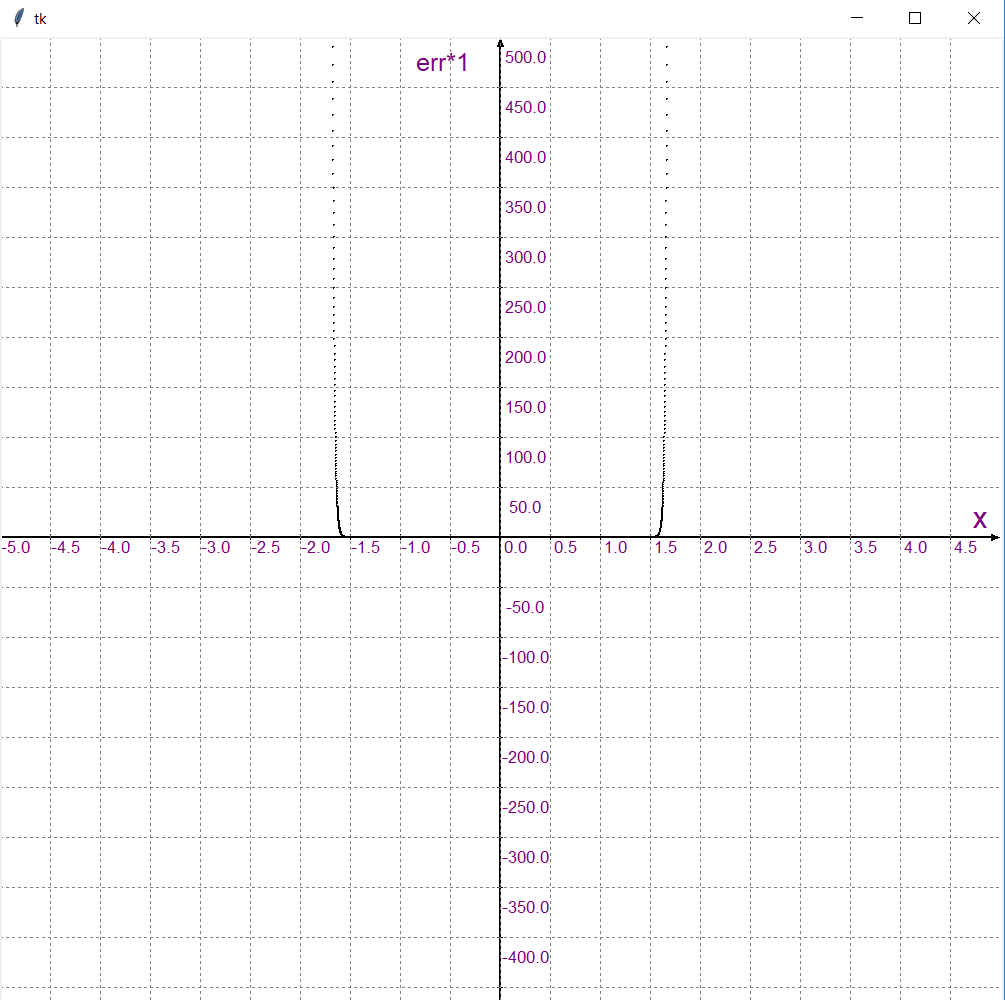
\includegraphics[width=\linewidth]{graph1}
		
		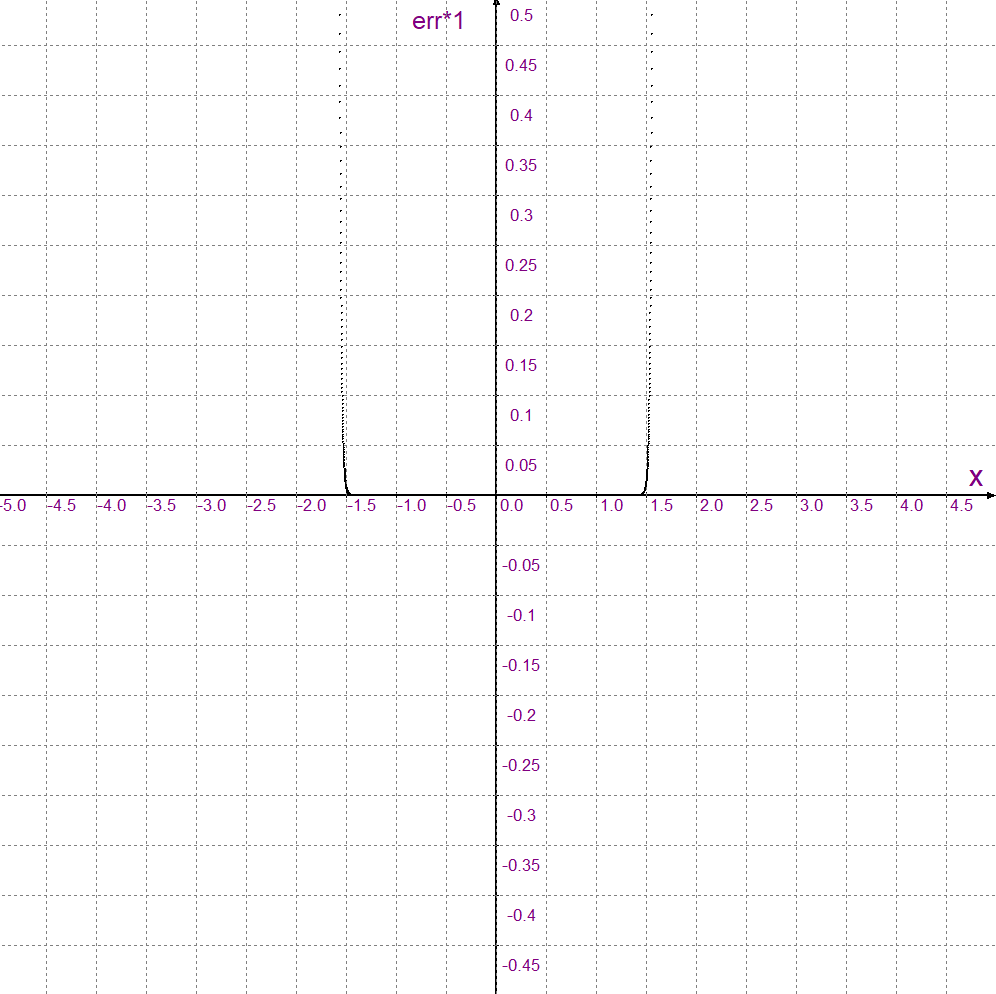
\includegraphics[width=\linewidth]{graph2} \\
		
		Видно резкое уменьшение точности \\
		Каждый график программа считала долго, около 10 минут. \\
	
\end{document}